%% Font size %%
\documentclass[11pt]{article}

%% Load the custom package
\usepackage{Mathdoc}

%% Numéro de séquence %% Titre de la séquence %%
\renewcommand{\centerhead}{Chapitre 2 : Probabilités Conditionnelles}

%% Spacing commands %%
\renewcommand{\baselinestretch}{1}
\setlength{\parindent}{0pt}

\begin{document}

\section{Probabilités conditionnelles dans un tableau}

\begin{definition}
On appelle \textbf{probabilité conditionnelle de $B$ sachant $A$}, la
probabilité que l'événement $B$ se réalise sachant que l'événement $A$
est réalisé. On la note : $P_A(B)$
\end{definition}


\begin{rappel}
  \begin{enuspaced}
  \item La probabilité d'un événement A est toujours comprise entre
    $0$ et $1$ : $0 \leq P(A) \leq 1$ ;
  \item Si $P(A) = 0$ : l'événement A ne se produit pas, il
    est impossible ;  
  \item Si $P(A) = 1$, l'événement se produit
    systématiquement ;  
  \item La somme des probabilités des évènements
    élémentaires est égale à $1$.
  \end{enuspaced}
\end{rappel}

\begin{remarque}
  Comme pour toutes les probabilités, on a : $0 \leq P_A(B) \leq 1$.
\end{remarque}

\begin{exercice}
  \textbf{Une entreprise de marketing a réalisé une étude sur 800 clients pour
  évaluer l'efficacité de deux types de campagnes publicitaires : la
  campagne A et la campagne B. Le tableau ci-dessous présente les
  résultats de l'étude, indiquant le nombre de clients qui ont réalisé
  un achat suite à ces campagnes :}

\begin{center}
  \begin{tabular}{|c|c|c|c|}
    \hline
    & \textbf{Acheté} & \textbf{Pas acheté} & \textbf{Total} \\
    \hline
    \textbf{Campagne A}   & 320             & 180                 & 500            \\
    \hline
    \textbf{Campagne B}   & 100             & 200                 & 300            \\
    \hline
    \textbf{Total}        & 420             & 380                 & 800            \\
    \hline
  \end{tabular}
\end{center}
    \begin{multicols}{2}
      \begin{enumerate}
      \item On choisit au hasard un client et on considère les
        événements suivants :
        \begin{itemize}
        \item \( A \) : « Le client a vu la campagne A. »
        \item \( G \) : « Le client a réalisé un achat. »
        \end{itemize}
        Calculer les probabilités suivantes :
        \begin{enumerate}
        \item \( P(A) \)
        \item \( P(G) \)
        \item \( P(G \cap A) \)
        \item \( P(\overline{G} \cap A) \)
        \end{enumerate}

        \item \begin{itemize}
        \item[a)] On choisit maintenant au hasard un client
          \textbf{ayant réalisé un achat}. Calculer la probabilité que
          ce client ait vu la campagne A sachant qu'il a réalisé un
          achat, \( P_G(A) \).
        \item[b)] On choisit maintenant au hasard un client
          \textbf{ayant vu la campagne B}. Calculer la probabilité que
          ce client ait réalisé un achat sachant qu'il a vu la
          campagne B, \( P_{\overline{A}}(G) \).
        \end{itemize}
      \end{enumerate}
    \end{multicols}
\end{exercice}

\section{Probabilités conditionnelles, formule}

\begin{propriete}
  $$P_A(B)=\dfrac{P(A \cap B)}{P(A)}$$
\end{propriete}

\begin{exercice}[0]
On tire une carte au hasard dans un jeu de 32 cartes. \\
Soit $A$ l'événement : « Le résultat est un pique ». \\
Soit $B$ l'événement : « Le résultat est un roi ». \\
Calculer $P_A(B)$, la probabilité que le résultat soit un roi sachant qu'on a tiré un pique.\\
\textbf{Correction.}
\begin{itemize}
\item On calcule $P(A)=\dfrac{8}{32}$ ; il y a 8 cartes piques dans le
  paquet ;
\item On calcule $P(B)=\dfrac{4}{32}$ ; il y a 4 rois dans le paquet ;
\item On calcule $P(A \cap B)=\dfrac{1}{32}$ ; il y a 1 seul roi de pique. 
\end{itemize}
Enfin, on applique la formule :
$$P_A(B)=\dfrac{P(A \cap B)}{P(A)}=\dfrac{\dfrac{1}{32}}{\dfrac{8}{32}}$$
Donc $P_A(B)=\dfrac{1}{8}$
\end{exercice}

\begin{remarque}
On peut retrouver intuitivement ce résultat. En effet, parmi les
piques, on a 1 chance sur 8 d'obtenir le roi.
\end{remarque}

\section{Arbre pondéré et probabilités totales}

\subsection{Propriétés}
\begin{propriete}
  Soit \( A \) et \( B \) deux événements avec \( P(A) \neq 0 \).
\[
P_{\overline{A}}(B) = 1 - P_{\overline{A}}(\overline{B})
\]
\[
P(A \cap B) = P(A) \times P_{\overline{A}}(B)
\]

\end{propriete}

\subsection{Construire un arbre pondéré}

\begin{exemple}
  \begin{center}
    \def\ArbreDeuxDeux{ $A$/$P(A)$/, $B$/$P_A(B)$/,
      $\overline{B}$/$P_A(\overline{B})$/,
      $\overline{A}$/$P(\overline{A})$/, $B$/$P_{\overline{A}}(B)$/,
      $\overline{B}$/$P_{\overline{A}}(\overline{B})$/ }
    \ArbreProbasTikz{\ArbreDeuxDeux}
  \end{center}
\end{exemple}

\begin{exercice}[0]
On donne : $P(A) = 0,4$ ; $P_A(B) = 0,3$ et $P_{\overline{A}}(B) = 0,2$. \\
Construire l'arbre pondéré représentant cette situation. \\
\textbf{Correction.}\\
On place dans notre arbre les probabilités que l'on connait :
\begin{center}
\def\ArbreDeuxDeux{ 
$A$/\num{0,4}/, 
$B$/\num{0,3}/,
$\overline{B}$/,
$\overline{A}$/, 
$B$/\num{0,2}/,
$\overline{B}$/ }
\begin{EnvArbreProbasTikz}
[Type=2x2,Fleche,EspaceNiveau=3,EspaceFeuille=1.5,PositionProbas=auto]%
{\ArbreDeuxDeux}
\end{EnvArbreProbasTikz}
\end{center}

On calcule les probabilités complémentaires : \\
$P(\overline{A})=1-P(A)=0,6$ ; $P_A(\overline{B})=0,7$ ; $P_{\overline{A}}(\overline{B})=0,8$.
\begin{center}
\def\ArbreDeuxDeux{ 
$A$/\num{0,4}/, 
$B$/\num{0,3}/,
$\overline{B}$/\textcolor{red}{\num{0,7}}/,
$\overline{A}$/\textcolor{red}{\num{0,6}}/, 
$B$/\num{0,2}/,
$\overline{B}$/\textcolor{red}{\num{0,8}}/ }
\begin{EnvArbreProbasTikz}
[Type=2x2,Fleche,EspaceNiveau=3,EspaceFeuille=1.5,PositionProbas=auto]%
{\ArbreDeuxDeux}
\end{EnvArbreProbasTikz}
\end{center}


On calcule les probabilités d'intersections : \\
$P(A \cap B) = P(A) \times P_{\overline{A}}(B)$
\begin{center}
\def\ArbreDeuxDeux{ 
$A$/\num{0,4}/, 
$B$/\num{0,3}/,
$\overline{B}$/\num{0,7}/,
$\overline{A}$/\num{0,6}/, 
$B$/\num{0,2}/,
$\overline{B}$/\num{0,8}/ }
\begin{EnvArbreProbasTikz}
[Type=2x2,Fleche,EspaceNiveau=3,EspaceFeuille=1.5,PositionProbas=auto]%
{\ArbreDeuxDeux}
\draw[red,->] (A24)--($(A24)+(2,0)$) node[right]
{$P(\overline{A} \cap \overline{B})=0,6 \times 0,8$} ;
\draw[red,->] (A21)--($(A21)+(2,0)$) node[right]
{$P(A \cap B)=0,4 \times 0,3$} ;
\end{EnvArbreProbasTikz}
\end{center}
\end{exercice}

\newpage
\subsection{Probabilités totales}

\begin{propriete}[Formule des probabilités totales]
$P(B)=P(A \cap B) + P(\overline{A} \cap B)$
\end{propriete}

\begin{demonstration}
\begin{center}
\def\ArbreDeuxDeux{ 
$A$/, 
$B$/,
$\overline{B}$/,
$\overline{A}$/, 
$B$/,
$\overline{B}$/ }
\begin{EnvArbreProbasTikz}
[Type=2x2,Fleche,EspaceNiveau=3,EspaceFeuille=1.5,PositionProbas=auto]%
{\ArbreDeuxDeux}
\draw[red,->] (A21)--($(A21)+(2,0)$) node[right]
{$P(A \cap B)$} ;
\draw[white] (A22)--($(A22)+(3,0)$) node[right]
{\textcolor{red}{+}} ;
\draw[red,->] (A23)--($(A23)+(2,0)$) node[right]
{$P(\overline{A} \cap B)$} ;
\draw[white] (A24)--($(A24)+(1,0)$) node[right]
{\textcolor{red}{$P(A \cap B)$ + $P(\overline{A} \cap B)$ = P(B)}} ;
\end{EnvArbreProbasTikz}
\end{center}
\end{demonstration}

\begin{exercice}[0][Utiliser la formule des probabilités totales]
Une entreprise propose une formation de gestion aux employés de différents services. Il a été observé que 40 \% des employés viennent du service commercial. À la fin de la formation, les résultats montrent que :
\begin{itemize}
\item Si un employé vient du service commercial, il réussit la formation dans 85 \% des cas ;
\item si un employé ne vient pas du service commercial, il réussit la formation dans 70 \% des cas.
\end{itemize}
On choisit de prendre ces fréquences observées comme probabilités pour
l'ensemble des employés et d'utiliser ces informations pour estimer
les chances de réussite à la formation. \\
On note respectivement \( C \) et \( R \) les événements « Être du service commercial » et « Réussir la formation ».
\begin{enu}
\item Un employé est choisi au hasard. Quelle est la probabilité qu'il réussisse la formation?
\item Si un employé a réussi la formation, quelle est la probabilité qu'il soit du service commercial?
\end{enu}
\end{exercice}

\section{Loi de Bernoulli}

\begin{definition}
  La loi de Bernoulli est une loi de probabilité qui décrit une
  expérience aléatoire ayant seulement deux issues possibles : un
  \textbf{succès} ou un \textbf{échec}.
\end{definition}

\begin{propriete}
  \begin{enu}
  \item La probabilité d'obtenir un succès est notée $p$.
  \item La probabilité d'obtenir un échec est notée $1 - p$.
  \item La variable aléatoire $X$ suivant la loi de Bernoulli peut
    prendre deux valeurs :
    \begin{itemize}
    \item $X = 1$ (succès) avec une probabilité $p$.
    \item $X = 0$ (échec) avec une probabilité $1 - p$.
    \end{itemize}
  \end{enu}
\end{propriete}

\begin{vocabulaire}
p est appelé le \textbf{paramètre} de la loi de Bernoulli.
\end{vocabulaire}

\begin{exemple}
  Lancer une pièce de monnaie est une expérience de Bernoulli où :
  \begin{itemize}
  \item Obtenir ``face'' est un succès avec une probabilité $p = 0.5$.
  \item Obtenir ``pile'' est un échec avec une probabilité
    $1 - p = 0.5$.
  \end{itemize}
\end{exemple}

\begin{center}
\tikzstyle{level 1}=[level distance=3cm, sibling distance=1.5cm]
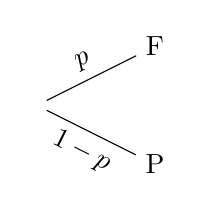
\begin{tikzpicture}[grow=right, sloped]
\node{}
child {node {P} edge from parent node[below] {$1-p$}}
child {node {F} edge from parent node[above] {$p$}};
\end{tikzpicture}
\end{center}

\section{Loi Binomiale}

\begin{definition}
La loi binomiale est une généralisation de la loi de Bernoulli qui
s'applique à une séquence de $n$ essais indépendants, chacun ayant une
probabilité de succès $p$. \\
Elle permet de modéliser le nombre total de succès obtenus parmi ces $n$ essais.
\end{definition}

\begin{propriete}
  \begin{enu}
  \item La loi binomiale est caractérisée par deux paramètres :
    \begin{itemize}
    \item $n$ : le nombre total d'essais.
    \item $p$ : la probabilité de succès pour chaque essai.
    \end{itemize}
  \item La variable aléatoire $X$ suivant la loi binomiale mesure le
    nombre de succès parmi les $n$ essais.
  \end{enu}
\end{propriete}

\begin{exercice}[0][Répétitions d’épreuves de Bernoulli]
On considère l'expérience suivante : \\
Une urne contient 3 boules blanches et 2 boules rouges. On tire au
hasard une boule et on la remet dans l'urne. \\
On répète l'expérience deux fois de suite.
\begin{enumerate}
\item Représenter l'ensemble des issues de ces expériences dans un arbre.
\item Déterminer les probabilités suivantes :
  \begin{enumerate}
  \item On tire deux boules blanches. 
  \item  On tire une boule blanche et une boule rouge. 
  \item  On tire au moins une boule blanche.
  \end{enumerate}
\end{enumerate}
\end{exercice}


\end{document}
%%% Local Variables:
%%% mode: LaTeX
%%% TeX-master: t
%%% End:
